\documentclass[a4paper,12pt]{article}

\usepackage{amsmath,amssymb,amsthm,multicol,tikz,enumitem}
\usepackage{hyperref}
\usepackage[margin=2cm]{geometry}
\usepackage{fancyvrb}
\usetikzlibrary{calc}

\newcommand\N{\mathbf{N}}
\newcommand\Q{\mathbf{Q}}
\newcommand\R{\mathbf{R}}
\newcommand\Z{\mathbf{Z}}

\newcommand\rem{\textup{rem}}

% Comment out one or the other

\newcommand\answer[1]{}
\newcommand\ans[1]{}
\newcommand\anscommand[1]{}
%\newcommand\answer[1]{${}$\\[5pt]{\color{blue}{#1}}\hfill{\color{blue}$\qed$}\\[-5pt]} 
%\newcommand\ans[1]{{\color{blue}{#1}}}
%\newcommand\anscommand[1]{#1}


\begin{document}

\begin{center}
{\bf\Huge Midterm} \\[5pt]
Data Structures and Algorithms, DatZ3168-EN\\
Wednesday, April 12, 2023\\[5pt]
\text{\em You must justify all your answers to get full credit}
\end{center}

\hrule
\vspace{2pt}
\hrule
\vspace{12pt}

\noindent
The problems can have somewhat different weights. The weights will be announced shortly.


\begin{enumerate}
% https://courses.cs.washington.edu/courses/cse373/13au/midterm1Solved.pdf

\item
For functions $f_1(n), f_2(n), f_3(n), f_4(n)$ defined below, 
give an asymptotic upper bound using Big-O notation.
Your answer should be {\em a tight bound} from the
following list (replacing the parameter $k$ with appropriate value):  
$O(n^k)$, $O(2^n)$, $O(2^{n!})$, $O(\log^k n)$, 
$O(n^k \log n)$, $O(1)$, $O(n^n)$, $O(n!)$, $O(n^k \log \log n)$, $O(n^k \log n)$. 
$O(n^k \cdot \log n \cdot \log \log n)$
(A tight bound means that giving a very large answer such as $O(2^{n!})$ 
won't result in many points, if it can be improved. 
Your answer should be a function of $n$ only, it must {\bf not} contain 
extra   parameters such as $k$.)

\begin{enumerate}
\item $f_1(n) = 5 \log n  \cdot \log \log n + 4 \log(n^3)$,
\item $f_2(n) = n \cdot \log(n!)$,
\item $f_3(n) = 8^{\log_7 n} + 15n$,
\item $f_4(n)$ is the running time of this Python function for argument $n$:
\begin{Verbatim}[frame=single,numbers=left]
def f4(n):
    for i in range(0, n):
        k = 1
        while k < i:
            k *= 2
            print("!")
\end{Verbatim}
\end{enumerate}

\vspace{5ex}

\begin{tabular}{ll}
(a) $f_1(n)$ & \rule{4cm}{0.4pt} \\[5ex]
(b) $f_2(n)$  & \rule{4cm}{0.4pt} \\[5ex]
(c) $f_3(n)$  & \rule{4cm}{0.4pt} \\[5ex]
(d) $f_4(n)$  & \rule{4cm}{0.4pt} \\[5ex]
\end{tabular}




\newpage

\item A very special kind of fractal tree can be drawn using the following 
pseudocode:

\begin{figure}[!htb]
\begin{minipage}{.35\textwidth}
\centering
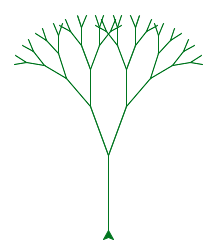
\includegraphics[width=2in]{fractal-tree.png}
\label{fig:fractal-tree}
\end{minipage}%
\begin{minipage}{0.65\textwidth}
\begin{Verbatim}
def drawBranch(length, angle):
    if length >= 1:
        drawLine(length);
        newLength = length / math.sqrt(2)
        newAngle1 = angle + 20
        newAngle2 = angle - 20
        drawBranch(newLength, newAngle1)
        drawBranch(newLength, newAngle2)
\end{Verbatim}
\end{minipage}
\end{figure}

The initial call is {\tt drawBranch(n, 90)} -- namely, 
the initial branch length is $n$ units long and the initial angle is 
$90^{\circ}$, i.e. vertical. At every subsequent level the branches
are shorter by a factor $\sqrt{2}$, and their angle differs
from the parent branch angle by $\pm 20^{\circ}$. 

\begin{enumerate}
\item Find the maximum depth of the recursion -- how many times 
{\tt drawBranch(...)} will recursively call itself before the 
length becomes less than $1$ unit. Express the maximum depth 
of the recursion tree with $n$ -- the parameter in the 
initial call. 
\item Find the number of calls to {\tt drawLine(...)} function
in terms of $n$. 
\item Denote the time complexity of this algorithm by $T(n)$
and find the asymptotic bound of $T(n)$ using the Master theorem. 
\end{enumerate}



\newpage

\item In this problem $a$ denotes the {\bf last} digit 
of your Student ID. 
Consider the graph shown in the figure below. 
Perform the {\em Breadth-first search} on this graph, 
starting from the node labeled $a$. 
If $a = 0$, then start from the node $10$. 

\begin{figure}[!htb]
\centering
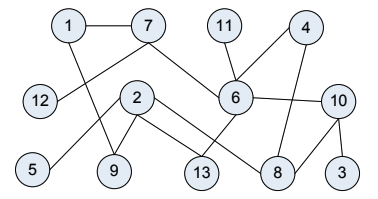
\includegraphics[width=3in]{undirected-graph.png}
\end{figure}


If it is possible to visit several neighboring nodes, 
pick the node with the smallest label. 
Whenever you visit the node, print its label. 

\begin{enumerate}
\item Redraw the graph showing the tree edges in bold or in 
a different color. 

%\vspace{30ex}

\item Write the node labels
in the order they are printed by the visit function.  
\end{enumerate}

\newpage

\item 

\begin{enumerate}
\item Explain the purpose of Binary Search Trees (BSTs). What alternative data
structures serve the same purpose? Compare their advantages and disadvantages.

%\vspace{30ex}

\item Let $a$, $b$ be the last two digits from your Student ID. Use them to compute values
$X, Y, Z, S, T, U$ (write them in the table). 

\vspace{2ex}

\begin{tabular}{ll|ll}
$S = 3 \cdot b$ & \rule{3cm}{0.4pt} & $T = 25+a$ & \rule{3cm}{0.4pt} \\[2ex]
$U = 2 \cdot a$ & \rule{3cm}{0.4pt} & $X = a$  & \rule{3cm}{0.4pt} \\[2ex]
$Y = (a+b)\,\text{mod}\,10$ & \rule{3cm}{0.4pt} & $Z = 5 \cdot (a+b)\,\text{mod}\,40$ & \rule{3cm}{0.4pt} \\[2ex]
\end{tabular}


\begin{figure}[!htb]
\begin{minipage}{.6\textwidth}
\centering
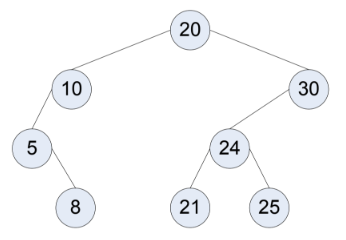
\includegraphics[width=3in]{binary_search_trees.png}
\label{fig:bsts}
\end{minipage}%
\begin{minipage}{0.4\textwidth}
$B.\text{\sc insert}(S)$\\
$B.\text{\sc insert}(T)$\\
$B.\text{\sc delete}(20)$\\
$B.\text{\sc show()}$\\
$B.\text{\sc insert}(U)$\\
$B.\text{\sc insert}(X)$\\
$B.\text{\sc delete}(25)$\\
$B.\text{\sc show()}$\\
$B.\text{\sc insert}(Y)$\\
$B.\text{\sc insert}(Z)$\\
$B.\text{\sc delete}(S)$\\
$B.\text{\sc show()}$
\end{minipage}
\end{figure}

The initial state of a binary tree $B$ is shown in the picture above. 
Run the above commands using the individualized 
numbers $X,Y,Z,S,T,U$. Whenever the command is $B.\text{\sc show()}$, 
draw the current state of the tree. (A command is ignored, 
if it tries to insert an existing node or to delete a non-existing one.)
\end{enumerate}







\newpage

\item File {\tt input.txt} contains some undirected graph. Its first line contains number $N$ -- the number of nodes in the graph. Nodes are enumerated with 
numbers $\{ 1,2,\ldots, N \}$. The second line contains number $E$ -- the number of edges in the graph. After that there are $E$ lines; each line contains two space-separated numbers $i$ $j$ (it defines an edge $\langle i, j \rangle$ where $i, j$ are two vertice numbers). To read numbers from {\tt input.txt}, you can use function {\tt readNumber()} returning a positive {\tt int} (or $-1$, if the end of the file is reached). 

\begin{enumerate}
\item 
Define a function {\tt canNumber()} returning {\tt bool} to determine, 
if the vertices in this graph can be assigned new integer numbers so that every two adjacent vertices $i$ and $j$ have their number total equal to an odd number.
(The new integer numbers can be picked arbitrarily -- they can repeat and
they are unrelated with the original numbers of the nodes.)
You can allocate any arrays you need and use integer variables. You can use all integer arithmetic operations including integer divison ({\tt 17 / 3 == 5}) 
and remainder operation ({\tt 17 \% 3 == 2}). 

\item Express the time complexity of the algorithm in part (a) 
in terms of $N$ and $E$. 
When there are several possible asymptotic bounds pick the smallest one. 
\end{enumerate}
\end{enumerate}

\end{document}

